\clearpage
\section{Procesevaluering}
%Processen   og   gruppens   refleksion   over   processen: Læringsprocessen,  teamroller,  samarbejdet  internt  i gruppen  og  med  vejleder,  projektarbejdsformen,  arbejdsformer, metoder, skriveprocessen, den tidsmæssige styring af projektet,ledelse af projektet, arbejdsfordeling i projektet m.m. Hvordan ville I gribe arbejdet an, hvis I skulle starte forfra?
Den overordnede proces for arbejdet er forløbet relativt uproblematisk, og har fulgt en lineær model for hvordan håndteringen af projektet skulle foregå. Figuren ses på figur \ref{fig:processen} og beskriver fra start til slut, hvilke faser gruppen skal igennem, for at ende op med et færdigt projekt. Gennem processen byggede vi også vores arbejde på idéerne ved "Unified Process" og "SCRUM", som skulle sikre, at gruppen arbejdede så effektivt med projektet som muligt.\\\\
Ved projektstarts-fasen begyndte vi i gruppen, at gøre os en idé om, hvordan vi vil arbejde med casen, og samtdigt fik vi alle lavet en analyse på vores tidligere projektarbejde, med henblik på at klargøre hvilke af Belbins team-roller gruppens medlemmer passer ind på. idéen ved at starte med at give hindanden roller, hjalp til at vi kunne uddelegere opgaver mere målrette, når man internt vidste hvilke styrker hvert medlem i gruppen besidder. Vi kunne ud fra vores nyerhvervede viden om hinandens styrker og svagheder, korrigerer hvem der så fik lov at arbejde med hvad, for at sikre at de forskellige opgaver ikke ville tage for lang tid. 
\begin{figure}[H]
    \centering
    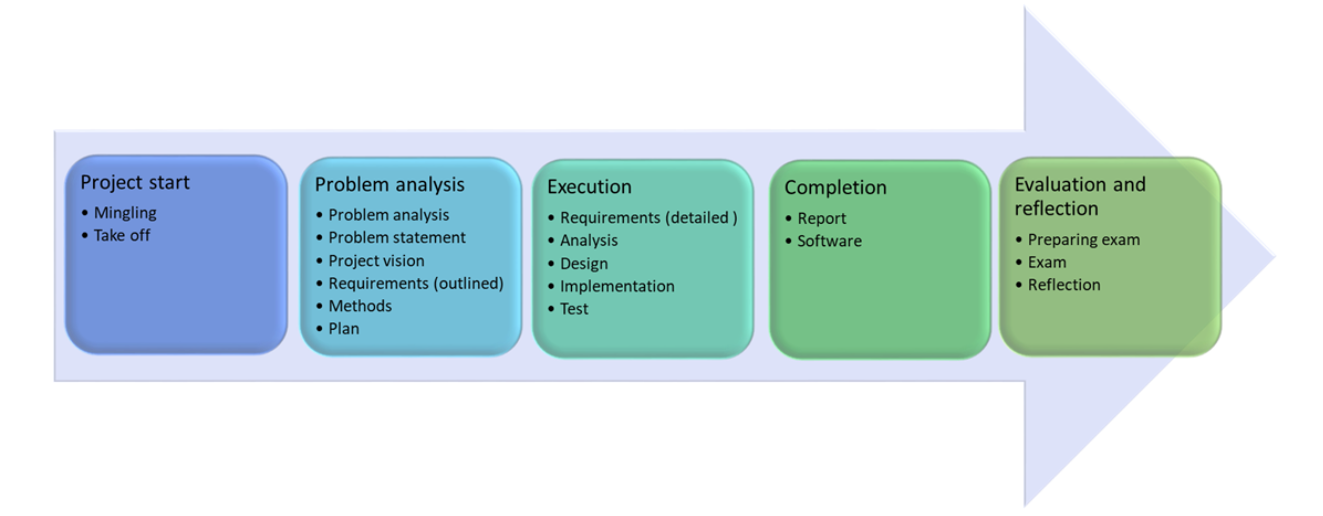
\includegraphics[width=1\textwidth]{images/processen.png}
    \caption{Processen for arbejdet med projektet}
    \label{fig:processen}
\end{figure}
Efter vores opstart, med tilrettelæggelsen af gruppen gik vi i gang med at analysere og løse problemet. Og til det fik gruppen bl.a. gjort brug af "UP" til udførelsen af dette. Unified Process er nemlig et sublimt instrument når det kommer til at arbejde med større projekter som dette. Gennem UP kunne vi dele vores projekt op i fire faser, som skulle overskueliggøre arbejdet med projektet. De fire faser og deres formål, ses beskrevet i tabel \ref{tab:UP_faser} og har hjulpet gruppen med at strukturere vores arbejde, så vi kunne arbejde målrettet med de forskellige elementer i både programmeringen af softwaresystemet og arbejdet med rapporten. 
        \begin{table}[H]
        \centering
        \begin{tabular}{|p{35mm}|p{105mm}|}
        \hline
            Inceptionsfasen & Målet med inceptionsfasen er, at finde ud af om projektet kan gennemføres, og fremskabe en business case. Derudover skal man her også bestemme systemets anvendelsesområde, samt udarbejde de vigtigste krav for systemet. I denne fase skal der også påpeges hvilke risici der er ved projektet.
        \\ \hline
            Elaborationsfasen & I denne fase er målet at skabe en kørbar arkitekturprototype og indfange størstedelen af brugsmønstrene. Dertil skal der laves en detaljeret plan for hvordan den næste fase (konstruktionsfasen) skal forløbe, samt et ekstra kig på hvor mange time der skal lægges i arbejdet, så man har styr på hvilke ressourcer der er til rådighed.
        \\ \hline
            Konstruktionsfasen & Målet med konstruktionsfasen er at færdiggøre brugsmønsteridentifikation, -realisering og -beskrivelser. Således at alle brugsmønstre er klart defineret, og noget man kan arbejde ud fra. Dertil skal analyse, design og tests færdiggøres. I denne fase skal der også holdes øje med at systemarkitekturen bliver overholdt.
        \\ \hline
            Transitionsfasen & I den sidste fase ligger arbejdets fokus på at rette fejl, og tilgængeliggøre systemet til brugeren. Her skal softwaren ændres, hvis der opstår uforudsete problemer, samt lave brugermanualer og anden dokumentation.
        \\ \hline
        \end{tabular}
            \caption{De fire faser i UP}
            \label{tab:UP_faser}
        \end{table}
Da gruppen så havde fået Unified Process på plads, lagde det også op til at vi benyttede os af SCRUM, til videre at skabe struktur i vores arbejde. %Hans skriv om SCRUM her
\\\\
SCRUM er et utroligt effektiv projekt styringsværktøj til agil udvikling af software, hvis det benyttes rigtig. Det var for gruppen første gang de skulle gør brug af SCRUM hvilket selvfølgelig er en svær opgave. Det viste sig også, at efter inceptionsdokumentet hvor gruppen havde skrevet et lille afsnit omkring brugen af SCRUM, at det ikke var nok og det krævede mere viden. Derfor satte gruppen sige for at læse en guide omkring SCRUM frameworket og skrive noter omkring hvordan hvert element er relevant for projektet.Dette dokument blev en rettesnor for hvordan gruppen ville benytte sig af SCRUM og hvem der indgår som de forskellige roller og hvordan hvert artefakt nås. 
Men det er én ting at skrive tanker og overvejelser ned. Det er en anden sag at anvende det, og det viste sig at have varierende effektivitet. Samlet set nåede gruppen at holde 4 Sprint. Første sprint var meget kort, og handlede om at lave struktur omkring objektopbygningen og få startet på en GUI. Dette sprint gik godt da opgaverne var delt ud i meget små bidder, som var hurtige at implementere. Samtidig var alle opgaver repræsenteret i et Sprint Backlog via et kanban board på GitHub. Dette gjorde det nemt at se hvad der skulle laves, hvem der havde ansvar for hvad, hvad der var blevet lavet og hvor meget der manglede. Alt i alt et godt sprint.\\\\
Sprint 2 var en anden sag. Da vi planlagde sprint 2 aftalte vi at det skulle handle om input og output til filer, hvilket er et fint mål. Det gik dog galt da opgaverne blev delt op på to punkter. Input/outpu på gui og read/write på filer.Dette er meget svært at forholde sig til. Ja der skal skrives til filer, men hvad kan én der sidder ikke og laver noget gå i gang med. Da kanban kun indeholder to punkter kan man ikke visualisere sig hvilket funktionalitet man skal implementere. Har forsvandt alle fordelene ved SCRUM da denne opdeling fjerne den inkrementele del af det, da det ender med at opgaven først er færdig når man kan skrive til alle filer. Derved bliver det en big-bang levering i stedet, hvilket kan være fint nok, men ikke når man arbejder agilt. Godt nok snakkede gruppen om ved starten af sprintet at "jaja vi skal nok dele den ud i forhold til brugsmønstre osv." men realiteten er, at hvis det ikke sker allerede ved planlægningen af sprintet, så bliver det ikke rigtig gjort. Det viser sig at være sjovere bare at kode end det er at lave diagrammer og brugsmønsterrealiseringer. Implmenteringen endte godt nok med at virke, men koden var rodet, forvirrende og dårligt struktureret. Dette havde kunne forbedres hvis der var brug noget mere tid på at lave design, inden kodningen tog fart. Kodeleveringen var langsom og dårlig. Alt i alt, et elendigt sprint.\\\\
Sprint 3 faldt efter midtvejsseminaret, hvor gruppen skulle fremlægge sit projekt, og få feedback, samt se andre fremlægge deres produkt, og give dem feedback. Dette blev lidt en øjenåbner da vi opdagede netop hvor dårlig strukturen på produktet var. Derfor var der enighed om, at sprint 3, handlede om restrukturering. Sprintplanlægningen gik til værks og det første der skulle klarlægges var et sprint mål. På gruppens GitHub blev sprintets mål defineret som: 

\textit{The sprint goal for this sprint is a restructured program using interfaces, facades and singleton patterns to ensure a well-defined three-layered architecture, and minimizes the use og static
As well as:
A relational Database has been structured and defined but not implemented in the program.}

Altså var der i sprintplanlægningen svaret på hvad spørgsmålet. Hvad skal laves. Gruppen diskuterede derfor hvorfor sprintet var vigtigt, og nåede til enighed om, at kravene der var sat skulle overholdes, og det gjorde den nuværende struktur ikke. Og sidst manglede sprøgsmålet hvordan. Vi kom fra et netop dårligt sprint med alt for få og for brede opgaver, så dette skulle absolut ændres. Der blev lagt fokus på design-patterns som singleton og facader som skulle implementeres. Der var fokus på at databasen skulle opsættes. Der skulle implementeres interfaces på de forskellige objekter og static metoder skulle gøre non-static. Der var mange opgaver, men de havde en størrelse der var til at bide over, og der var nok opgaver til at alle kunne sidde med noget samtidig. Næsten lige som SCRUM skal være. Og endda da der ikke var flere opgaver, startede en dialog i gruppen og fandt hurtigt frem til en opgave der var relevant at gå i gang med, så spildtid blev minimeret inden sprintet var ovre. Der blev undervej f.eks. tilføjet en opgave om, at man skal kunne querye database, som ikke var inkludere i starten. Derved blev der leveret et inkrement mere end hvad var planlagt, for at minimere idle-time. Det endte med at være et udemærket sprint hvor gruppen opnåede en langt bedre struktur på produktet, særligt med hensigt om at overholde tre-lags-modellen.\\\\
4. sprint var sidste sprint og der var massere at lave. Gruppen havde lært fra tidligere fejl, at opgaver ikke skal være for abstrakte og store. Dette var der meget fokus på, samt at bruge kanban endnu mere. Jo mere der bliver tilføjet til kanban, jo nemmere er det at have overblik over hvad status er pt. Hver gang et nyt issue, eller en ny fejl/mulighed opstod, blev der, i stedet for at gå i gang med en ny opgave så man sad med to, skrevet en ny note på kanban, så fokus kunne forblive på den nuværende opgave, og dermed færdiggøres. Derved kan resten af gruppen også gå i gang med disse i stedet for at sidde stille. 4 Sprint blev dog stort, og der blev leveret flere inkrementer. Måske var sprintet en smule for stort, men projektet var også ved at være ovre så gruppen var nødt til at dedikere meget tid til det. Og det endte med at gruppen fik opnået stort set alle opgaver og havde en god grundfunktionalitet, der var nem at udvide på og som samtidig overholdte tre-lags-modellen. 4. sprint var et godt sprint, og havde klart det bedste fokus på opgavestruktureringen.
Alt i alt har gruppen lært utroligt meget om SCRUM. Både hvordan det absolut ikke skal bruges, men også omvendt; hvordan det kan udnyttes på en effektiv måde. Vi i gruppen har i hvert fald opdaget hvor effektivt det kan være, hvis man tager sig tid til at lave ordentlige sprint-planlægninger.
\\\\ %Afsluttende ord om samarbejdet
Samarbejdet i gruppen har generelt set været godt, og vi har alle komplimenteret hindanden på en god måde. Gruppen har været gode til at overholde de indbyrdes aftaler, hvilket resulterede i et miljø hvor vi alle kunne stole på hinanden, og stole på at de ting der skulle laves, blev gjort udførligt. Den gode gruppe dynamik, blev også hjulpet godt på vej af en håndfuld sociale arrangementer. Disse sociale arrangementer har nemlig lagt bund for at gode venskaber på tværs af gruppen kunne gro. 

Udover dette har vejledermøderne også været super brugbare, og "on point", når det kommer til at blive hjulpet i den rigtige retning. Det har ikke været ved alle gruppens samtaler med vores vejleder Henrik, at der har været lige meget at diskutere, men når der endelig var et problem, havde Henrik altid svaret. Hvilket var super betryggende, og gav gruppen rig mulighed for at arbejde videre, med et positivt mindset og et klart overblik, efter hvert vejledermøde.
\\\\
For videre at uddybe vores Belbin-roller, er det også lige værd at komme ind på, hvordan de forskellige roller gruppens medlemmer besidder, har hjulpet til udførelsen af projektet. I tabel \ref{tab:Belbin_roller} ses listen over Gruppens belbin-roller. Samlet set skaber vores kombination af roller både fordele for gruppens arbejde, men der er også svagheder forbundet hertil.
        \begin{table}[H]
        \centering
        \begin{tabular}{|p{30mm}|p{50mm}|}
        \hline
            Jonas Beltoft & Afslutter\newline
                            Specialist \newline
                            Idémand
        \\ \hline
            Hans Pedersen & Afslutter \newline
                            Analysator \newline
                            Specialist
        \\ \hline
            Victor Bruun & Formidler \newline
                           Kontaktskaber \newline
                           Afslutter
        \\ \hline
            Jesper Bork & Kontaktskaber \newline
                          Koordinator \newline
                          Formidler
        \\ \hline
            Casper Stillinge & Specialist \newline
                               Organisator \newline
                               Afslutter
        \\ \hline
            Peter Ratgen & Formidler \newline
                           Afslutter \newline
                           Specialist
        \\ \hline
        \end{tabular}
            \caption{Gruppens Belbin-roller}
            \label{tab:Belbin_roller}
        \end{table}
Af styrker kan det påpeges at fem ud af de seks gruppemedlemmer er afsluttere, hvilket vil sige, at gruppen er god til at få en opgave afsluttet og gjort færdigt, så længe strukturen er på plads. Dertil er fire ud af seks medlemmer specialister. Dette bidrager til at gruppen besidder en bred viden, og samtidigt er selvstartende. Tre ud af seks er formidlere, som er med til at skabe et godt samarbejde i gruppen.

Modsat kan svaghederne ligeledes findes i at der er mange afsluttere, men ingen opstartere i gruppen. Det betyder at gruppen har haft problemer med at komme i gang med opgaverne, indtil én af gruppens medlemmer påtager sig en lederrolle. Ligeledes er de mange afsluttere og få koordinatorer samt opstartere, en svær kombination. I og med at der er få gruppemedlemmer, der instinktivt ville lave forarbejdet, så der var en klar plan, som afslutterne kunne gøre færdigt. Gruppen har også en del specialister, som har resulteret i, at der ofte var blevet lagt fokus i mindre detaljer, som havde en lav indvirken i det overordnede projekt. Dette problem kunne have været løst hvis der eventuelt var en organisator mere, som kunne holde styr på afslutterne og korrigere arbejdet i den rigtige retning. Dertil kunne det også have været godt med en idémand mere, så de to idémænd kunne spare med hinandens idéer og løfte dem. 
\\\\
Afsluttende er det værd at nævne, at alle i gruppen havde en unik baggrund, når det kom til kodekendskab og udvikling af software, hvilket betød at nogle medlemmer i gruppen er mere rutineret i miljøet end andre. Dette har dog ikke været et problem, da det blev set som en mulighed for at lære noget mere, og blive stærkere på områder man individuelt set ikke ville føle sig tryg i normalt. Det har været en lærerig oplevelse, og vi, gruppens medlemmer, er alle blevet klogere, både på samarbejde og hvor vi hver især står fagligt, efter denne opgave.